\documentclass{beamer}
\title{Algorithms and Complexity, weeks 1-5 key points}
\author{Sam Barrett}
\newcommand{\qs}{q_{\texttt{start}}}
\newcommand{\qh}{q_{\texttt{halt}}}
\newcommand{\U}{\mathcal{U}}
\newcommand{\N}{\mathbb{N}}
\newcommand{\DT}{\mathbf{DTIME}}
\usepackage{mdframed,amsmath,amssymb,amsfonts,tikz,mathtools}
\usetikzlibrary{shapes,arrows,calc,positioning,backgrounds}

\newmdtheoremenv{thesis}{Thesis}
\newcommand\defeq{\stackrel{\mathclap{\normalfont\mbox{def}}}{=}}


\begin{document}

\begin{frame}
\titlepage
\end{frame}

\begin{frame}[allowframebreaks]
  \frametitle{Turing machine basics}

  \begin{itemize}
    \item Turing machines are \textbf{precise models of computation}
    \item First tape of a Turing machine is \textbf{always} a read-only \textbf{input tape}.
    \item The $k^{th}$ tape is always the output tape
    \item The output tape is also considered a work tape
    \item The alphabet of a TM is denoted as \(\Gamma\), or sometimes $\Sigma$, it is \textbf{finite}.
    \item Each tape must always start with the \textit{left-of-tape} symbol, $\rhd$
    \item $\{ 0,1 \} ^{*}$ is the set of bitstrings, with $\varepsilon$ denoting the empty string.
  \end{itemize}

  \framebreak{}

  In a single stage of computation a TM may:
  \begin{itemize}
    \item read the character at any/all of the tape heads
    \item writes a character at any/all of the work tape heads
    \item may move any/all tape heads to the left or to the right. (tapes are not recursive)
  \end{itemize}

\end{frame}

\begin{frame}
\frametitle{what does it mean to say that $M$ \textbf{computes} $f$?}

It means that for every bitstring $x \in \{ 0,1 \}^{*}$, if we start in state $\qs$ with the initial configuration showing $x$ (meaning $x$ appears on the input tape and and the work tapes are blank), when we run $M$, we eventually reach $\qh$ with the output tape showing $\rhd$ on the leftmost cell and then the bitstring $f(x)$ followed by all blanks.

\end{frame}

\begin{frame}
  \frametitle{Computable functions}
  \framesubtitle{Basics}

  \begin{definition}(Computable functions)
    We say a function $f : \{ 0,1 \} ^{*} \rightarrow \{ 0,1 \} ^{*}$ is \textbf{computable} if there exists some Turing machine that computes it.
  \end{definition}

  No variation of Turing machine affects this fact.

  \begin{thesis}[ Church's Thesis (informal) ]
    any algorithm that computes a function from bitstrings to bitstrings can be converted into a Turing machine that computes the same function
  \end{thesis}
\end{frame}

\begin{frame}[allowframebreaks]
  \frametitle{Boolean functions, languages and Decidability}

  \begin{definition}[Language]
    A \textit{language} can be defined as any set of words
  \end{definition}

  \begin{definition}[Boolean Function]
    A \textbf{boolean function} is a function of the form: $f : \{ 0,1 \}^{*} \rightarrow \{ 0,1 \} $. Noting that the output is a single bit rather than a bitstring.
  \end{definition}

  \color{red} There is a one-to-one correspondence between languages and boolean functions.\color{black}
\begin{itemize}
  \item For a given boolean function $f$ the corresponding language is the set of bitstrings $\mathcal{X}$ s.t. $\forall x\in \mathcal{X}, f(x) = 1$
  \item For a language $L$, the corresponding boolean function sends $x$ to 1 if $x \in L$ and to $0$ otherwise.
\end{itemize}

This allows us to treat boolean functions, languages and decision problems as essentially the same thing.

A decision problem is said to be \textbf{decidable} when the corresponding boolean function is \textbf{computable}. I.e. given a language $L$, for $L$ to be decidable there must exist some Turing machine that will start with a bitstring $x$ and will run continuously until it halts and upon halting there will be a $1$ on the output tape if $x \in L$ or $0$ if it is not in the language.
\end{frame}

\begin{frame}
  \frametitle{Data Representation}
  \begin{itemize}
    \item We can encode many real-life data types as bitstrings, but not all. (e.g. Real numbers cannot)
    \item We can encode multiple inputs as a single bitstring.
  \end{itemize}
\end{frame}

\begin{frame}
  \frametitle{Code as Data}
  \begin{itemize}
    \item We can not only encode many data types as bitstrings, we can encode program code or even other Turing machines as bitstring inputs to a TM as our TMs are essentially 6-tuples (see full notes for formal definition).
    \item We can therefore say that for \textbf{any} bitstring \(\alpha\) we can construct a corresponding TM:  $M_{\alpha}$
  \end{itemize}
\end{frame}

\begin{frame}
  \frametitle{The Universal Turing Machine, $\U$}

  $\U$ is a Turing machine interpreter written as a Turing machine. It takes 2 inputs (encoded as a single input): $\alpha$ and $x$, where $\alpha$ is the bitstring describing the machine to be interpreted and $x$ is the bitstring input.

  We define $\U$ as having 4 tapes and the basic alphabet of $\{ \rhd, \Box, 0,1 \} $.  Intuitively, $\U$ works by simulating the $M_{\alpha}$ by \textit{providing} it with the 3 non-input tapes to $M_{\alpha}$ as its input, work and output tape respectively.
\end{frame}

\begin{frame}[allowframebreaks]
  \frametitle{Diagonalisation \& the Halting problem}

  \begin{problem}(The halting problem)
    the set of pairs $\langle \alpha,x \rangle $ (encoded as a single bitstring) such that the machine $M_{\alpha}$ executed on input $x$ halts.
  \end{problem}

  \framebreak
  Turing's proof is as follows:

    \begin{proof}
    Suppose that $N$ is a machine that solves the halting problem.

    We can convert it into a machine $N'$ that, given $x$, runs forever if $\langle x,x \rangle \in \texttt{HALT} $ (i.e. the machine $M_{x}$ executed on $x$ halts), and halts otherwise.

    We know $N' = M_{\alpha }$ for some $\alpha $, i.e. there exists some bitstring $\alpha $ that represents our new machine, as we know every machine can be represented as a bitstring.

    Running $N'$ on $\alpha$ halts if it runs forever and runs forever if it halts.

    We have derived a contradiction.


  \end{proof}

  \framebreak

  More intuitively, we can consider the described machine $N$ as:
    \begin{center}
    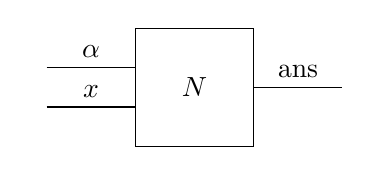
\begin{tikzpicture}

        \node [rectangle,draw,minimum size = 15mm] (N) at (2,2) {$N$};


        \node (i1) at (0,2.25) {};
        \node (i2) at (0,1.75) {};

        \draw (i1) -- node[above] {$\alpha $} (1.25,2.25);
        \draw (i2) -- node[above] {$x$} (1.25,1.75);

        \node (o1) at (4,2) {};

        \draw (N) -- node[above] {ans} (o1);
    \end{tikzpicture}
  \end{center}

  Where  \texttt{ans} is whether $N$ halts.

  We can then construct the wrapper $N'$ as:


    \begin{center}
    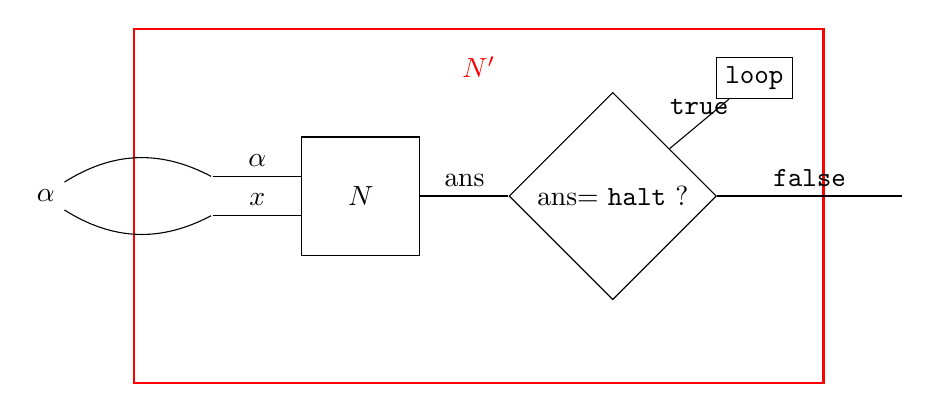
\begin{tikzpicture}
        %\draw [help lines] (-5,-5) grid (10,10);

        \node [rectangle,draw,minimum size = 15mm] (N) at (2,2) {$N$};


        \node (i1) at (0,2.25) {};
        \node (i2) at (0,1.75) {};

        \draw (i1) -- node[above] {$\alpha $} (1.25,2.25);
        \draw (i2) -- node[above] {$x$} (1.25,1.75);

        \node (o1) at (4,2) {};

        \draw (N) -- node[above] {ans} (o1);

        \draw[red,thick] ($(o1.north west)+(4,2)$)  rectangle node[above = 1.5cm of o1] {$N'$} ($(i2.south east)+(-1,-2)$);

        \node (i3) at (-2,2) {$\alpha $};

        \draw (i3) edge[bend right] (0.1,1.75);
        \draw (i3) edge[bend left] (0.1,2.25);
        \node [draw, diamond] (q) at (5.2,2){ans= \texttt{halt} ?};

        \node [draw,rectangle] (loop) at (7,3.5) {\texttt{loop} };

        \node (o2) at (9,2) {};

        \draw (q) -- node[above] {\texttt{false} } (o2);
        \draw (q) -- node[above] {\texttt{true} } (loop);


    \end{tikzpicture}
    \end{center}
    \textbf{Where the outermost $\alpha$ is the bitstring of $N'$}

    You can clearly see that if $N$ were to halt then $N'$ would hang. We can therefore derive a contradiction as if we pass $N'$ into $N'$ it would have to half if it hangs and vice versa!


  \end{frame}

  \begin{frame}
    \frametitle{Upper bound notation}

    \begin{itemize}
      \item     If we have two function $f : \N \rightarrow \N$ and $g : \N \rightarrow \N$
      \item We say that $f(n)$ is $O(g(n))$ is $f$ is \textbf{no bigger} than $g$ up to \textbf{a}  constant factor, i.e. given a constant $c$ and a value $n_{0}$ s.t. $\forall n, n \geq n_{0}$ we have:

            \[
            f(n) \leq c\cdot g(n)
            \]

      \item We say that $f(n)$ is $o(g(n))$ if $f$ is \textbf{not as big as }$g$, even up to any constant factor. Or, if, \textbf{for any} $\varepsilon > 0$, there is a $n_{0}$ s.t. $\forall n, n\geq n_{0}$ we have:

            \[
            f(n) \leq \varepsilon \cdot g(n)
            \]

            Whenever $f(n)$ is $o(g(n))$ is it also $O(g(n))$, this is the case if you take $c$ to be 1

    \end{itemize}


  \end{frame}

  \begin{frame}
    \frametitle{Lower bound notation}

    \begin{itemize}
      \item     If we have two function $f : \N \rightarrow \N$ and $g : \N \rightarrow \N$
      \item We say that $f(n)$ is $\Omega(g(n))$ when $g(n)$ is $O(f(n))$
      \item We say that $f(n)$ is $\omega(g(n))$ when $g(n)$ is $o(f(n))$
      \item We say that $f(n)$ is $\Theta(g(n))$ when it is \textbf{both} $O(g(n))$ and $\Omega(g(n))$

            This informally means \textit{$f(n)$ and $g(n)$ are the same, up to a constant factor}
    \end{itemize}
  \end{frame}

  \begin{frame}
    \frametitle{Time complexity}

    \begin{definition}[Worst case running time:]

      The running time of a machine $M$ is the time taken from the input state, where $x$ sits on the input tape and the other tapes are blank, to reach the halt state ($q_{\texttt{halt} }$).

      For any number $n$, we define $\texttt{WT}_{M}(n) $ to be the \textbf{worst case} running time for an input of length $n$.
    \end{definition}

    \begin{definition}[$\mathbf{DTIME} $ classes]

      $\mathbf{DTIME} $ is a \textbf{set} of complexity classes.

      A complexity class can be thought of as a set of decision problems (or languages or boolean functions...)

      $\DT(n^{2})$ is an example of a complexity class. A function $f : \{ 0,1 \}^{*} \rightarrow \{ 0,1 \} $ is in $\DT(n^{2})$ when there is some machine that decides it and has worst case running time in $O(n^{2})$
    \end{definition}

    This definition is robust.


  \end{frame}

  \begin{frame}
    \frametitle{Polynomial Time}

    We can define the complexity (super) class of \textbf{polynomial time decision problems} as:

    \[
      \mathbf{P} \;\; \defeq \;\; \bigcup_{k\geq1}\mathbf{DTIME} (n^{k})
    \]

  \end{frame}

  \begin{frame}
    \frametitle{Exponential Time}

    We can define the complexity class of \textbf{exponential time decision problems} as:

    \[
      \mathbf{EXP} \;\; \defeq \;\; \bigcup_{k\geq 1} \mathbf{DTIME} (2^{n^{k}})
    \]

    It is clear that $\mathbf{P} \subseteq \mathbf{EXP} $


  \end{frame}

  \begin{frame}
    \frametitle{Space Complexity}

    We can extend this notion to space usage of our models.

    The space usage of a Turing Machine for an input $x$ is the number of cells on the \textbf{work tapes} that are non-blank at \textbf{some point during execution}. Blank cells are ignored as there are infinitely many of these.

  \end{frame}

  \begin{frame}
    \frametitle{The $\mathbf{SPACE}$ Complexity class}

    The spacial analogue for $\mathbf{DTIME} $ we say a problem is in $\mathbf{SPACE} (n^{2})$ if there exists a TM which decides it and has worst case space usage in $O(n^{2})$
  \end{frame}

  \begin{frame}
    \frametitle{$\mathbf{L}$ \& $\mathbf{PSPACE}$ }

    We can define logarithmic space, $\mathbf{L} $ which defines the set of things that can be computed with a machine using a logarithmic number of cells (relying on the fact we do not count the input tape cells).

    \begin{definition}[Logspace]
      \[
        \mathbf{L} \;\; \defeq \;\; \mathbf{SPACE}(\log n)
      \]

      We can also define polynomial space, $\mathbf{PSPACE} $:

      \begin{definition}[polynomial space]
        \[
          \mathbf{PSPACE} \;\; \defeq \;\; \bigcup_{k \geq 1}\mathbf{SPACE}(n^{k})
        \]

        It is clear that $\mathbf{L} \subseteq \mathbf{PSPACE} $
      \end{definition}

    \end{definition}
  \end{frame}
  \begin{frame}
    \frametitle{Space vs. Time}
    We can show that, in \textbf{all cases}, space complexity is less than or equal to time complexity, meaning also that:

    \[
      \mathbf{P} \subseteq \mathbf{PSPACE}
    \]

    \small\textit{See notes for a proof}

    Equally we can show that, in all cases, time is less than or equal to exponentiated space, i.e.

    \[
      \mathbf{L} \subseteq \mathbf{P}
    \]

    \small\textit{See notes for a proof}
  \end{frame}

  \begin{frame}
    \frametitle{Nondeterministic Time Complexity}
    We can informally define $\mathbf{NP} $ as:

    \begin{definition}[NP - informal]
     Problems for which \textbf{checking} a solution is easy
   \end{definition}

   We have two methods for formally defining $\mathbf{NP} $:

   \begin{enumerate}
     \item Using certificates

     \item Using nondeterministic Turing machines
   \end{enumerate}

   For both, we will use the example of $n$-Sudoku. Where $n$ describes the dimension of the grids.

   Let $\mathbf{SUD} $ be the set of \textbf{solvable} $n$-Sudoku puzzles.

   Given a puzzle $x$, a solution \textbf{certifies} that $x \in \mathbf{SUD}$ The size of a solution is polynomial in $|x|$. The time taken to check a candidate solution is also polynomial in $|x|$

 \end{frame}

 \begin{frame}
   \frametitle{Using Certificates}
   \begin{definition}[NP - certificates]
     A language $L$ is in $\mathbf{NP} $ if there is a polytime machine for checking polynomially-sized certificates of $L$, precisely:

     If there is a polynomial, $p$, which gives the size of a candidate certificate, and a polynimal time machine $M$ s.t. $\forall x \in \{ 0,1 \} ^{*}$, where $x$ is a bitstring representing an $n$-Sudoku puzzle, the following are equivalent:

     \begin{itemize}
       \item $x \in L$

       \item There is some bitstring $u$ representing a solution to $x$, of length $p|x|$ s.t. $M \langle x,u \rangle =1$
     \end{itemize}

     In these cases we say that $u$ certifies that $x \in L$
   \end{definition}
 \end{frame}

 \begin{frame}[allowframebreaks]
   \frametitle{Using Nondeterministic Turing Machines}
   Nondeterministic TMs are TMs which have two transition functions $\delta_{0}, \delta_{1}$ and an additional accepting state $q_{\text{accept}}$. It starts at $\qs$ and follows transitions from either transition function until it reaches either $\qh$ or $q_{\text{accept}}$, at which point no more transitions take place.
   \framebreak{}
   \begin{definition}[NP - Nondeterministic TMs]
     A language $L$ is in $\mathbf{NP} $ when there is a polytime nondeterministic machine $M$, s.t. $\forall x \in \{ 0,1 \} ^{*}$ the following are equivalent:

     \begin{itemize}
       \item $x \in L$
       \item When $M$ is executed on input $x$, there is some sequence of transitions that lead to $q_{\text{accept}}$
     \end{itemize}
   \end{definition}
 \end{frame}

 \begin{frame}
   \frametitle{Nondeterministic Space complexity}
   What does it mean for a nondeterministic Turing machine (NDTM) to be in nondeterministic polynomial space complexity?

   Let $M$ be a NDTM, it is in polyspace if $\texttt{WS}_{M} $ is $O(n^{k})$ for some $k\geq 1$.

   The worse case space complexity is polynomial, therefore $\mathbf{NPSPACE} $ is the class of languages that can be decided by a polyspace NDTM. We can therefore say:

   \[
     \mathbf{PSPACE} \subseteq \mathbf{NPSPACE}
   \]

   in the same way that we say

   \[
     \mathbf{P} \subseteq \mathbf{NP}
   \]


 \end{frame}

 \begin{frame}
   \frametitle{Savitch's Theorem: $\mathbf{PSPACE} = \mathbf{NPSPACE}  $}

   We can show this equivalence using a special case of Savitch's theorem.

   Suppose we have a NDTM, $M$ and for an input size $n$ the space usage is polynomial in $n$. The length of a configuration of $M$ is also polynomial in $n$.

   Let us say for $n\geq 1000$ a configuration has a length at most $7n^{18}$.

   Consider the digraph representing all $\leq 2^{7n^{18}}$ configurations of $M$ and the transitions linking them.

   With this graph, we want to, using a space-efficient algorithm, work out if there is a path from the start configuration to any accepting configuration. If such a path exists, we know that the input is accepted.
 \end{frame}

 \begin{frame}[allowframebreaks]
   \frametitle{Finding a path space-efficiently}
   We find this required path by generalising our problem.

   Given nodes $s$ and $t$ and a number $k$, how much space do we use when deciding whether there is path of length $\leq 2^{k}$ from $s\rightarrow t$? We will assume we have some function which calculates this, $D$, where $D(k)$ returns this result.

   We will now argue, by induction, that $D(k) \leq k \cdot 7n^{18}$

   For each configuration $t$, check if $t$ is accepting and whether there is a path from the start configuration to $t$.

   Storing $t$ requires at most $7n^{18}$ bits, $D(7n^{18}$ bits to check for the path, $\therefore$ at most $7n^{18} + D(7n^{18})$ bits total.

   This is polynomial, as is required by Savitch's theorem.

   \framebreak{}

   \begin{proof}
     \underline{Base Case} If $k =0$, just check if $s=t$

     \underline{Inductive step} Find whether there is a path from $s$ to $t$ of length $\leq 2^{k+1}$:

     \begin{enumerate}
       \item For each node $z$, test whether there is a path from $s$ to $z$ of length $\leq 2^{k}$ and a path from $z$ to $t$ of length $\leq 2^{k}$
       \item By our inductive hypothesis, this takes $\leq k \cdot 7n^{18}$ cells, plus a further $7n^{18}$ cells to store $z$, totalling $\leq (k+1) \cdot 7n^{18}$

             $\therefore D(k+1) \leq (k+1) \cdot 7n^{18}$

             $\therefore \forall k D(k) \leq k \cdot 7n^{18}$
     \end{enumerate}


   \end{proof}


 \end{frame}
\end{document}
